\section{The Online Alignment Framework}

To allow the calibration and alignment tasks to operate, they have been embedded
in the online system in terms of data flow and control flow.

\subsection{Data Flow}

All of the tasks make use of events that have been accepted by the HLT1 stage of
the High Level Trigger. The alignment tasks require events with specific
content such as decays of \decay{\Dz}{\kaon\pion} or \decay{\jpsi}{\mup\mum}, or
tracks with specific properties. The calibration tasks have no requirements on
the event content, but do require a sufficient number of events to fill the
distributions used to obtain the calibration constants.

Events for the alignment tasks are selected by dedicated selections that are
part of HLT1 and, based on acceptance by these selections, written to files on
the hard-drives installed in the farm nodes. The number of events written to
files across the farm is tracked and once a sufficient number for a given task
has been accumulated, the tasks writing events are stopped, until a new sample
is required. The Velo alignment requires 

Approximately a kilohertz of events accepted by HLT1 is transferred over the
network to dedicated tasks that processes as many of these events as they
can. These tasks provide the distributions required to perform the calibration,
and write them to files. The files are written every fifteen minutes and at
least once per run, which is a period of data-collection up to an hour long.

\subsection{Control Flow}

\begin{figure}[h]
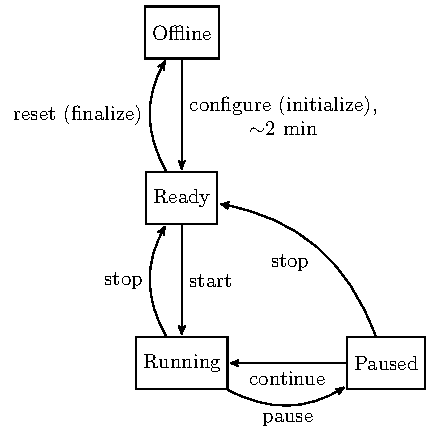
\includegraphics[width=5cm]{../figures/FSM}
\caption{Finite state machine that defines the behaviour of the alignment
  tasks.}
\label{fig:FSM}
\end{figure}

The Outer Tracker calibration and RICH refractive index calibration tasks run
independently from ECS and wait for the files containing the distributions they
require. Once a file becomes available for a given run, the calibration
algorithms are triggered to process the distributions, and if a new set of
calibration constants is created, write these to a file. The ECS is then
informed of the availability of the new versions and which run(s) these
correspond to.

The execution of the alignment tasks is under the control of the LHCb Experiment
Control System (ECS), and is implemented as a finite state machine, which is
shown in \cref{fig:FSM}. Once FSM reaches the initial ``READY'' state, it will
loop from ``READY''$\to$``RUNNING''$\to$``PAUSED''$\to$``READY'' until it stops
when a convergence criterium is satisfied.

The task that steers the iterations is called the iterator and the tasks that
analyze the data are called the analyzers; both tasks follow the same sequence
of states. When all tasks are in the ``READY'' state, the iterator makes an
initial set of alignment constants available to the analyzers and then updates
its state to ``RUNNING''. The analyzers are then sent the ``start'' command,
update their state to ``RUNNING'' and start analyzing their data. Each analyzer
that has completed processing its data updates its state to ``PAUSED'', and once
they have all reached this state, they are sent the ``stop'' command and update
their state to ``READY''. The iterator is then sent the ``pause'' command,
collects and combines the output produced by the analyzer tasks and either
indicates that conversion has been reached by updating its state to ``READY'',
or that further iteration is required by producing a new set of constants and
updating its state ``RUNNING''. If the iterator decides that the process has
converged and the changes in the alignment constants are above a given
threshold, it writes the new alignment constants to a file and announces the new
version to the control system.
